\pdfminorversion=4
\documentclass[aspectratio=169]{beamer}

\mode<presentation>
{
  \usetheme{default}
  \usecolortheme{default}
  \usefonttheme{default}
  \setbeamertemplate{navigation symbols}{}
  \setbeamertemplate{caption}[numbered]
  \setbeamertemplate{footline}[frame number]  % or "page number"
  \setbeamercolor{frametitle}{fg=white}
  \setbeamercolor{footline}{fg=black}
} 

\usepackage[english]{babel}
\usepackage[utf8]{inputenc}
\usepackage{tikz}
\usepackage{courier}
\usepackage{array}
\usepackage{bold-extra}
\usepackage{minted}
\usepackage[thicklines]{cancel}
\usepackage{fancyvrb}

\xdefinecolor{dianablue}{rgb}{0.18,0.24,0.31}
\xdefinecolor{darkblue}{rgb}{0.1,0.1,0.7}
\xdefinecolor{darkgreen}{rgb}{0,0.5,0}
\xdefinecolor{darkgrey}{rgb}{0.35,0.35,0.35}
\xdefinecolor{darkorange}{rgb}{0.8,0.5,0}
\xdefinecolor{darkred}{rgb}{0.7,0,0}
\definecolor{darkgreen}{rgb}{0,0.6,0}
\definecolor{mauve}{rgb}{0.58,0,0.82}

\title[2022-09-08-chess-scientific-python-ecosystem]{Adoption of Python and modern software practices \\ in high energy physics}
\author{Jim Pivarski}
\institute{Princeton University -- IRIS-HEP}
\date{September 8, 2022}

\usetikzlibrary{shapes.callouts}

\begin{document}

\logo{\pgfputat{\pgfxy(0.11, 7.4)}{\pgfbox[right,base]{\tikz{\filldraw[fill=dianablue, draw=none] (0 cm, 0 cm) rectangle (50 cm, 1 cm);}\mbox{\hspace{-8 cm}\includegraphics[height=1 cm]{princeton-logo-long.png}\hspace{0.1 cm}\raisebox{0.1 cm}{\includegraphics[height=0.8 cm]{iris-hep-logo-long.png}}\hspace{0.1 cm}}}}}

\begin{frame}
  \titlepage
\end{frame}

\logo{\pgfputat{\pgfxy(0.11, 7.4)}{\pgfbox[right,base]{\tikz{\filldraw[fill=dianablue, draw=none] (0 cm, 0 cm) rectangle (50 cm, 1 cm);}\mbox{\hspace{-8 cm}\includegraphics[height=1 cm]{princeton-logo.png}\hspace{0.1 cm}\raisebox{0.1 cm}{\includegraphics[height=0.8 cm]{iris-hep-logo.png}}\hspace{0.1 cm}}}}}

% Uncomment these lines for an automatically generated outline.
%\begin{frame}{Outline}
%  \tableofcontents
%\end{frame}

% START START START START START START START START START START START START START

\begin{frame}{Subject of this talk: a rough assortment of things}
\vspace{0.5 cm}

\begin{itemize}\setlength{\itemsep}{0.5 cm}
\item Adoption of Python in high energy physics (HEP)

\vspace{0.1 cm}
\begin{itemize}\setlength{\itemsep}{0.25 cm}
\item How Python is used in HEP, trend toward Python for data analysis
\end{itemize}

\item Adoption of ``modern software practices'' (devops)

\vspace{0.1 cm}
\begin{itemize}\setlength{\itemsep}{0.25 cm}
\item Source control: git/GitHub/GitLab
\item Automated tests: continuous integration (CI), continuous deployment (CD)
\item Modularity of packages: Lego-style analysis
\item Package management: pip, conda
\item Environment encapsulation: venv, conda, Docker
\item Social structures: silos versus mixing
\end{itemize}

\end{itemize}
\end{frame}

\begin{frame}{Is Python part of that ``modern''?}
\large
\vspace{0.25 cm}
Python is leading every programming language popularity index.
\vspace{0.25 cm}
\begin{columns}[t]
\column{0.33\linewidth}
\centering Tiobe
\vspace{0.1 cm}
\includegraphics[width=\linewidth]{PLOTS/python-rankings-tiobe-2022.png}
\column{0.33\linewidth}
\centering PYPL
\vspace{0.1 cm}
\includegraphics[width=\linewidth]{PLOTS/python-rankings-pypl-2022.png}
\column{0.33\linewidth}
\centering Google Trends
\vspace{0.1 cm}
\includegraphics[width=\linewidth]{PLOTS/python-rankings-googletrends-2022.png}
\end{columns}
\vspace{0.25 cm}
\begin{columns}[t]
\column{0.5\linewidth}
\centering GitHut
\vspace{0.1 cm}
\includegraphics[width=\linewidth]{PLOTS/python-rankings-githut-2022.png}
\column{0.45\linewidth}
\centering StackOverflow
\vspace{0.1 cm}
\includegraphics[width=\linewidth]{PLOTS/python-rankings-stackoverflow-2022.png}
\end{columns}
\end{frame}

\begin{frame}{Is Python part of that ``modern''?}
\large
\vspace{0.25 cm}

And this is a recent thing, too.

\vspace{0.25 cm}
\href{https://www.tiobe.com/tiobe-index/}{\textcolor{blue}{Tiobe index}}'s top 3 or 4 for the past 35 years:

\renewcommand{\arraystretch}{1.25}
\begin{center}
\begin{tabular}{c l l}
1987 & C, Lisp, Prolog                 & \\
1992 & C, C++, Pascal                  & Python exists \\
1997 & C, C++, (Visual) Basic          & Python is \#28 \\
2002 & Java, C, C++, (Visual) Basic    & Python is \#12 \\
2007 & Java, C, C++, (Visual) Basic    & Python is \#7 \\
2012 & Java, C, C++, C\#               & Python is \#8 \\
2017 & Java, C, C++, C\#               & Python is \#5 \\
2022 & Python, C, Java, C++            & Python is \#1 \\
\end{tabular}
\end{center}
\end{frame}

\begin{frame}{Not all programmers are data analysts: what about us?}
\vspace{0.25 cm}

Google search trends for language name + ``analytics'' or ``machine learning.''

\includegraphics[width=\linewidth]{PLOTS/analytics-by-language.pdf}
\end{frame}

\begin{frame}{Not all data analysts are physicists: what about us?}
\vspace{0.25 cm}

Regex matches to all Computing in High Energy Physics (CHEP) titles and abstracts.

\vspace{-0.1 cm}
\begin{center}
\only<1>{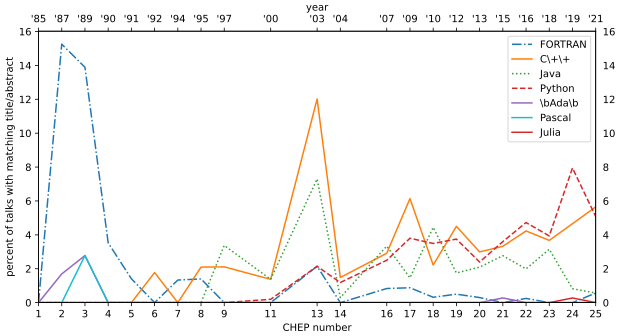
\includegraphics[width=0.95\linewidth]{PLOTS/chep-papers-language.pdf}}\only<2>{\includegraphics[width=0.95\linewidth]{PLOTS/chep-papers-language-shaded.pdf}}
\end{center}
\end{frame}

\begin{frame}{Lucas Taylor, summary of data analysis track, CHEP 2001}
\vspace{0.25 cm}

\mbox{ } \hfill \includegraphics[width=0.82\linewidth]{PLOTS/chep-2001-python.png} \hfill \mbox{ }
\end{frame}

\begin{frame}{}
\vspace{1 cm}
\Large

\begin{center}
But note the emphasis on ``glue'' and ``configuration,''

\vspace{0.1 cm}
not the process of analyzing data.

\vspace{1 cm}
How do physicists {\it use} Python now?
\end{center}
\end{frame}

\begin{frame}{Analysis of 11\,635 GitHub repos created by 2\,172 physicists}
\vspace{0.25 cm}

Software for the CMS experiment is on GitHub and all CMS physicists need to fork it. Using that, we can identify all of those physicists' non-fork, public repositories.

\vspace{0.2 cm}

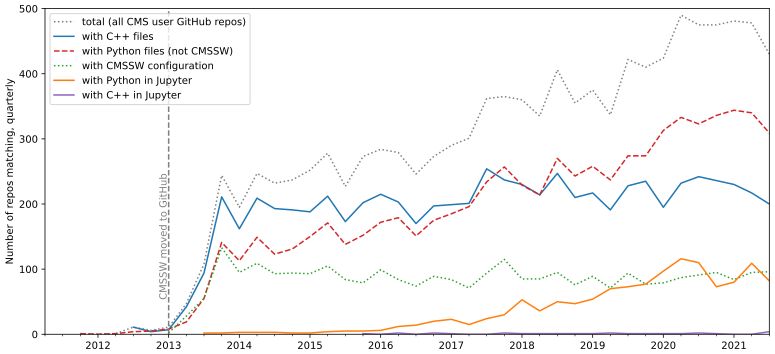
\includegraphics[width=\linewidth]{PLOTS/gihub-language-fullstudy.pdf}
\end{frame}

\begin{frame}{Analysis of 11\,635 GitHub repos created by 2\,172 physicists}
\vspace{0.25 cm}

By regex searching for ``\mintinline{python}{import [A-Za-z_][A-Za-z_0-9]*}'' etc., we can count the number of physicist repositories that use different packages over time.

\vspace{0.2 cm}

\includegraphics[width=\linewidth]{PLOTS/gihub-package-fullstudy.pdf}
\end{frame}






\end{document}
